\documentclass[pdf]{beamer}
%\documentclass[handout]{beamer} % handout 

\usepackage[german]{babel}
\usepackage[utf8]{inputenc}
\usepackage[autostyle=true,german=quotes]{csquotes}
\usepackage{graphicx} 
\usepackage{listings}

% IST NUR FUER DAS INHALTSVERZEICHNIS!
\usepackage{multicol}
% FUER NORMALE SPALTEN SIEHE TUTORIAL BEAMER Charles T. Batts

\mode<presentation>{

    \usetheme{Warsaw}
	\usecolortheme{seahorse}

    \setbeamertemplate{section in toc}[sections numbered]
	\setbeamertemplate{subsection in toc}[subsections numbered]

	%\setbeamertemplate{itemize items}[default]
	%\setbeamertemplate{enumerate items}[default]

	\beamersetuncovermixins{\opaqueness<1>{15}}{\opaqueness<2->{5}}
	%  zeigt das jeweils naechste ausgeblendete Element an

%	\setbeamercovered{transparent}
	% zeigt ausgeblendete Elemente transparent an
	\setbeamertemplate{navigation symbols}{}
	% To remove the navigation symbols from the bottom of all slides uncomment this line
}

\title[Referat LB Aufgabe 3]{Deduktive Datenbanken und Unifikation}  
\subtitle{Familien-Datenbank}

\institute{Hochschule für Angewandte Wissenschaften Hamburg}

\author{Uwe Krause}

%\date{\today} 
\date{Wintersemester 2016/17}

\subject{Computer Science}

% Die Bilddatei mit dem Namen (Ohne Dateiendung) "Hawhamburg-logo" wird 
% mit dem Namen "university-logo" deklariert
\pgfdeclareimage[height=.8cm]{university-logo}{img/Hawhamburg-logo}

% das zuvor deklarierte Bild kann verwendet werden
\logo{\pgfuseimage{university-logo}} % Nutzt das Logo auf jeder Seite



\AtBeginSection[] { % fuegt eine Folie vor Beginn eines neue Kapitels ein
	\mode<beamer> { % fuegt fur Handout KEIN Inhaltsverzeichnis vor jedem Kapitel ein
		\begin{frame}{\contentsname}
		\begin{multicols}{2}
		\tableofcontents[currentsection]
		\end{multicols}
		\end{frame}
	}
}



\begin{document}

	\begin{frame}{}
		% Die "Titelseite" ist die allererste Folie,
		% Titel und Name der Praesentation und das alles
		\titlepage
	\end{frame}

	% Komplettes Inhaltsverzeichnis einmal am Anfang
	\begin{frame}{\contentsname}
			\begin{multicols}{2}
	\tableofcontents[]
			\end{multicols}
	\end{frame}



	\section{Einleitung}

	\subsection{Erklärung der Aufgabe}

	\begin{frame}[plain]{Erklärung der Aufgabe}
		\begin{figure}[!ht]
  		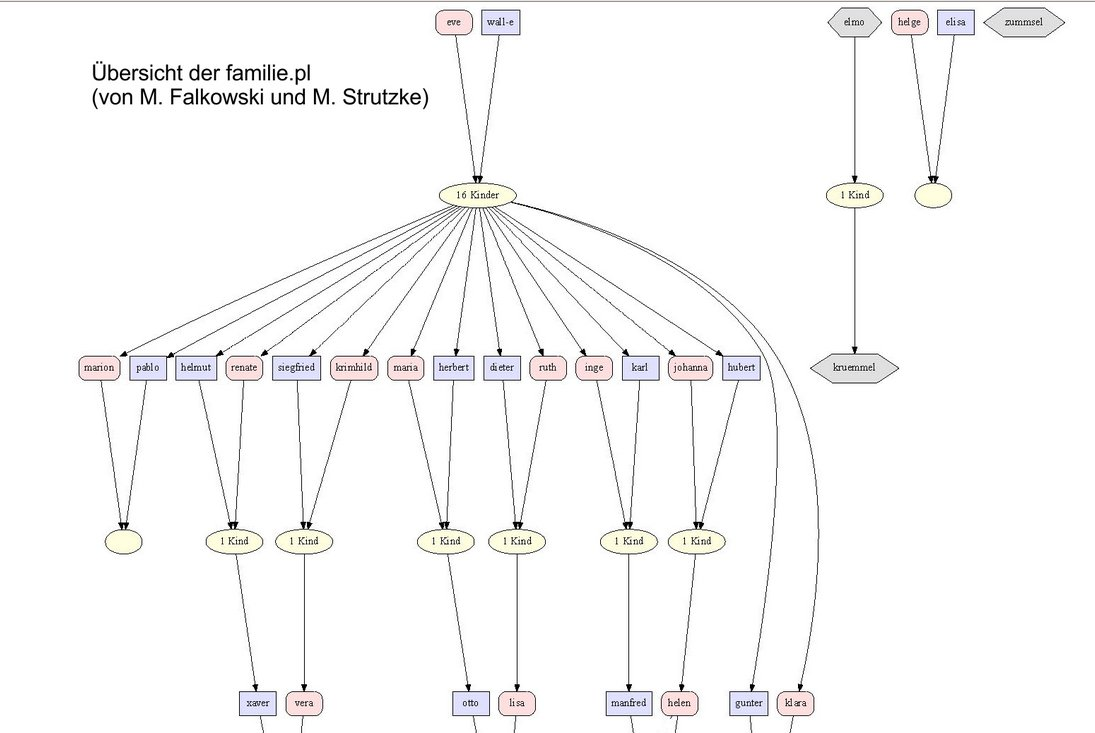
\includegraphics[height=\textheight]{img/stammbaum}
	\end{figure}
	\end{frame}


	\subsection{Natürlichsprachige Lösungen}

	\begin{frame}[allowframebreaks]{Natürlichsprachige Lösungen}
		\begin{description}[Nachkomme]
				\item[Vorfahre] Eine Person ist ein Vorfahre einer anderen Person,
				wenn er Elternteil der anderen Person ist, oder wenn es einen Menschen gibt,
				der ein Vorfahre der Person ist und ein Elternteil der anderen Person ist.
				\item[Nachkomme] Ein Nachkomme einer Person ist jede Person, die die Person als Vorfahren hat.
				\item[Geschwister] Zwei Menschen sind Geschwister, wenn sie mindestens einen gemeinsamen Elternteil haben.
				\item[Schwester] Eine Person, die weiblich und ein Geschwisterteil einer anderen Person ist, ist eine Schwester.
				\item[Bruder] Eine Person, die männlich und ein Geschwisterteil einer anderen Person ist, ist ein Bruder.
				\item[Eheleute] Im normalen Sprachgebrauch impliziert die Aussage \enquote{X ist mit Y verheiratet},
				dass Y ebenfalls mit X verheiratet ist.
				\item[Uroma] Eine Person ist Uroma einer anderen Person,
				wenn sie weiblich und ein Elternteil einer Oma oder eines Opas der anderen Person ist.	

			\end{description}
	\end{frame}
	


	\section{Beispiellösung Geschwister}
	
	\subsection{Umformung: natürlichsprachig}
	
	\begin{frame}{Umformung: natürlichsprachig}
		\begin{exampleblock}{Geschwister}
			Zwei Menschen sind Geschwister, wenn sie mindestens einen gemeinsamen Elternteil haben.
		\end{exampleblock} \pause

		\begin{block}{etwas förmlicher}
			Zwei (unterschiedliche) Personen sind Geschwister,
			wenn es eine andere Person gibt, die Elternteil beider Personen ist.
		\end{block} \pause

		\begin{alertblock}{Formale Definition}
			Für alle Personen
			X und Y gilt,
			X und Y sind Geschwister
			wenn
			es eine Person E gibt, für die gilt
			E ist Elternteil von X
			und
			E ist Elternteil von Y.
		\end{alertblock}

	\end{frame}
	
	\subsection{Umformung: Prädikatenlogik}
		
	\begin{frame}[t]{Umformung: Prädikatenlogik}

		\begin{figure}[!ht]
  		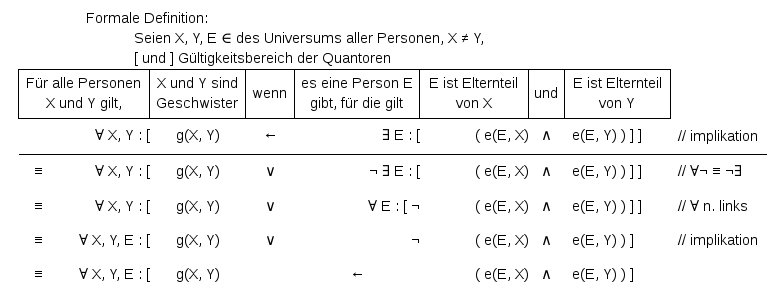
\includegraphics[width=\textwidth]{img/umformung}
		\end{figure}\pause\pause
		
		\centering
		geschwister(X, Y) :- elternteil(E, X), elternteil(E, Y), \\ 
		X \textbackslash == Y.
		
	\end{frame}
		
		


	\section{Konsistenzprüfung}
	\subsection{findall}

	\begin{frame}[t]{findall}

		\begin{figure}[!ht]
  		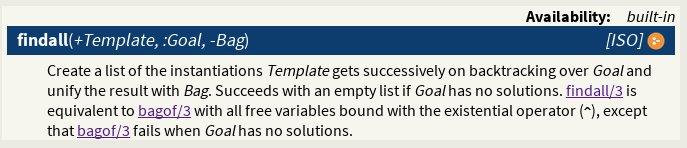
\includegraphics[width=\textwidth]{img/findall} \\
  		Auszug aus der Dokumentation\footnote{www.swi-prolog.org}
		\end{figure}
		
		Erstellt eine Liste aller Belegungen (Substitutionen) von Variablen,
		die eine gegebene Anfrage erfolgreich auswerten lassen.


	\end{frame}


	\section{Anfragen}
	
	
	\subsection{Anfragen}
	
	\begin{frame}{Anfragen}
		\begin{block}{?- Stimmt es dass...?}
			Eine Anfrage (\enquote{goal}) kann als \enquote{Stimmt es, dass ...?} Frage gesehen werden.

		\end{block}
		Um die Erfüllbarkeit dieser Frage zu beweisen, wird nach dem Resolutionsverfahren vorgegangen.
		\footnote{Zuerst wird behauptet, die Anfrage sei unter allen Umständen (Belegungen) wahr (Tautologie).
		Da mit dem Resolutionsverfahren aber nur Widersprüche bewiesen werden können,
		wird diese Behauptung zu einem Widerspruch negiert.} \\
		Gemeinsam mit den vorher definierten Fakten und Regeln (in allquantifizierter Form)
		kann der Widerspruch bewiesen werden.

	\end{frame}

	\section{\enquote{Gibt es eine Person, die zugleich männlich und weiblich ist?}}
	\subsection{Behauptung}
	\begin{frame}{Behauptung}
	
		\begin{figure}[!ht]
  		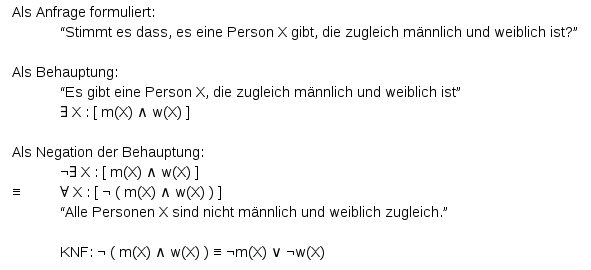
\includegraphics[width=\textwidth]{img/behauptung}
		\end{figure}
		 
	\end{frame}
	
	\subsection{Resolution}
	\begin{frame}{Resolution}

		\begin{figure}[!ht]
  		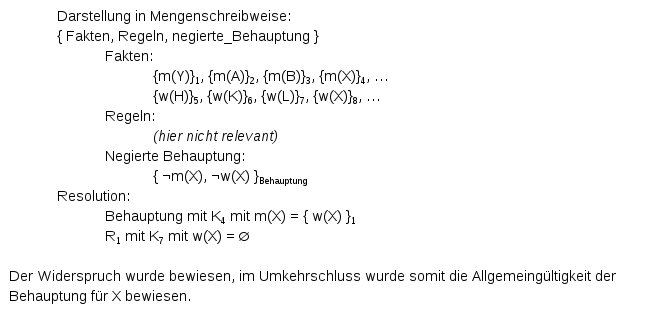
\includegraphics[width=\textwidth]{img/resolution}
		\end{figure}

	\end{frame}

	\appendix

\section<presentation>*{\appendixname}

	\subsection<presentation>*{Literaturangaben \& weiterführende Literatur}

		\begin{frame}{Literaturangaben}


			\begin{thebibliography}{}

				\beamertemplatebookbibitems
				% Anfangen sollte man mit Übersichtswerken.

				\bibitem{Goehner}
					H. Göhner / B. Hafenbrak
					\newblock {\em{Arbeitsbuch Prolog}}


				\beamertemplatearticlebibitems
				% Vertiefende Literatur kommt später. Die Liste sollte kurz sein.

				\bibitem{Klauck}
					\href{http://users.informatik.haw-hamburg.de/~klauck/pub/LB/lbskript.pdf}C. Klauck
					\newblock { \em Logik, HAW Hamburg }

				\bibitem{Richter}
					 \href{http://www-hm.ma.tum.de/archiv/in2/ss02/literatur.html}{J. Richter-Gebert}
					 \newblock{ \em Skript zur Vorlesung \enquote{Logik}, ETH Zürich}

				
				\setbeamertemplate{bibliography item}[online]
				\bibitem{Doku}
					 \href{http://www.swi-prolog.org/pldoc/doc_for?object=findall/3}{swi-prolog.org}
					 \newblock{ \em Dokumentation}

			\end{thebibliography}

		\end{frame}




\end{document}